% This file was created with tikzplotlib v0.10.1.
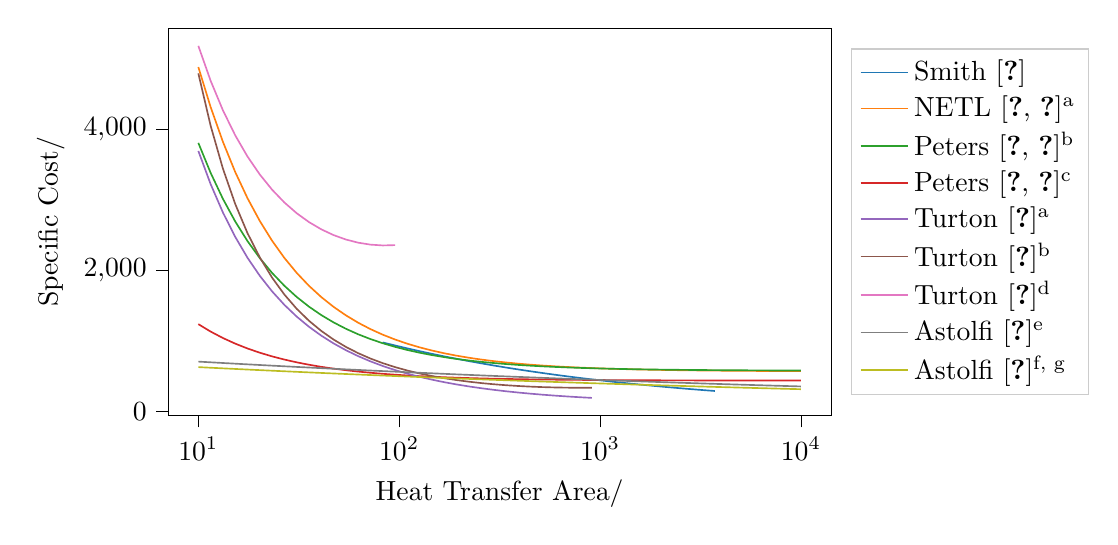
\begin{tikzpicture}

\definecolor{crimson2143940}{RGB}{214,39,40}
\definecolor{darkgray176}{RGB}{176,176,176}
\definecolor{darkorange25512714}{RGB}{255,127,14}
\definecolor{forestgreen4416044}{RGB}{44,160,44}
\definecolor{goldenrod18818934}{RGB}{188,189,34}
\definecolor{gray127}{RGB}{127,127,127}
\definecolor{lightgray204}{RGB}{204,204,204}
\definecolor{mediumpurple148103189}{RGB}{148,103,189}
\definecolor{orchid227119194}{RGB}{227,119,194}
\definecolor{sienna1408675}{RGB}{140,86,75}
\definecolor{steelblue31119180}{RGB}{31,119,180}

\begin{axis}[
legend cell align={left},
legend style={fill opacity=0.8, draw opacity=1, text opacity=1, draw=lightgray204, at={(1.03, 0.5)}, anchor=west},
log basis x={10},
tick align=outside,
tick pos=left,
unbounded coords=jump,
x grid style={darkgray176},
xlabel={Heat Transfer Area/\unit{\square\m}},
xmin=7.07945784384138, xmax=14125.3754462276,
xmode=log,
xtick style={color=black},
xtick={0.1,1,10,100,1000,10000,100000,1000000},
xticklabels={
  \(\displaystyle {10^{-1}}\),
  \(\displaystyle {10^{0}}\),
  \(\displaystyle {10^{1}}\),
  \(\displaystyle {10^{2}}\),
  \(\displaystyle {10^{3}}\),
  \(\displaystyle {10^{4}}\),
  \(\displaystyle {10^{5}}\),
  \(\displaystyle {10^{6}}\)
},
y grid style={darkgray176},
ylabel={Specific Cost/\unit{\USD\per\square\m}},
ymin=-58.2302966684393, ymax=5436.36210712615,
ytick style={color=black},
width=10cm, height=6.5cm
]
\addplot [semithick, steelblue31119180]
table {%
10 nan
11.5139539932645 nan
13.2571136559011 nan
15.2641796717523 nan
17.5751062485479 nan
20.2358964772516 nan
23.2995181051537 nan
26.8269579527973 nan
30.8884359647748 nan
35.5648030622313 nan
40.9491506238043 nan
47.1486636345739 nan
54.2867543932386 nan
62.5055192527397 nan
71.9685673001152 nan
82.8642772854684 978.089325766849
95.4095476349994 934.94633301296
109.854114198756 893.706354405864
126.48552168553 854.285449017691
145.634847750124 816.603378509635
167.683293681101 780.583443812749
193.069772888325 746.152329012661
222.29964825262 713.239952120446
255.954792269954 681.779322425923
294.705170255181 651.706404143013
339.322177189533 622.959986069631
390.693993705462 595.481556996813
449.843266896944 569.215186613468
517.947467923121 544.10741166437
596.362331659464 520.107127129654
686.6488450043 497.165482204322
790.60432109077 475.235780866043
910.298177991522 454.273386828855
1048.11313415469 434.235632689297
1206.79264063933 415.08173308007
1389.49549437314 396.772701654433
1599.85871960606 379.271271732378
1842.06996932672 362.541820447058
2120.95088792019 346.550296237072
2442.05309454865 331.264149537033
2811.76869797423 316.652266525331
3237.45754281764 302.68490579425
3727.59372031494 289.333637813533
4291.93426012878 nan
4941.71336132383 nan
5689.86602901829 nan
6551.28556859551 nan
7543.12006335462 nan
8685.11373751352 nan
10000 nan
};
\addlegendentry{Smith \cite{Smith2005}}
\addplot [semithick, darkorange25512714]
table {%
10 4885.49356223176
11.5139539932645 4317.65532109122
13.2571136559011 3824.4813502097
15.2641796717523 3396.15414726098
17.5751062485479 3024.14709981291
20.2358964772516 2701.05474798861
23.2995181051537 2420.44536565712
26.8269579527973 2176.73292552089
30.8884359647748 1965.06589933787
35.5648030622313 1781.2306796498
40.9491506238043 1621.56770045463
47.1486636345739 1482.8985870566
54.2867543932386 1362.46288488239
62.5055192527397 1257.86310773836
71.9685673001152 1167.01701159692
82.8642772854684 1088.11614383716
95.4095476349994 1019.58984278896
109.854114198756 960.073970927493
126.48552168553 908.383759297079
145.634847750124 863.490222584449
167.683293681101 824.499675341607
193.069772888325 790.635941592409
222.29964825262 761.224903673543
255.954792269954 735.681082727175
294.705170255181 713.495983706187
339.322177189533 694.227972878659
390.693993705462 677.493486325386
449.843266896944 662.95939441998
517.947467923121 650.336370292987
596.362331659464 639.373130267556
686.6488450043 629.851431612303
790.60432109077 621.581728032783
910.298177991522 614.399396416418
1048.11313415469 608.16145971755
1206.79264063933 602.743740745843
1389.49549437314 598.038390199127
1599.85871960606 593.951739731817
1842.06996932672 590.402437320412
2120.95088792019 587.319827807223
2442.05309454865 584.642546384185
2811.76869797423 582.317297017543
3237.45754281764 580.297791495806
3727.59372031494 578.543827980824
4291.93426012878 577.020490718917
4941.71336132383 575.697454980892
5689.86602901829 574.548383394537
6551.28556859551 573.550401652534
7543.12006335462 572.683643158808
8685.11373751352 571.930853548711
10000 571.277047210301
};
\addlegendentry{NETL \cite{Loh2002, Adams2021}\textsuperscript{a}}
\addplot [semithick, forestgreen4416044]
table {%
10 3809.47868383405
11.5139539932645 3384.39307314783
13.2571136559011 3015.20138544882
15.2641796717523 2694.55420558777
17.5751062485479 2416.06848291715
20.2358964772516 2174.20046535035
23.2995181051537 1964.13534114689
26.8269579527973 1781.6913915477
30.8884359647748 1623.23674624868
35.5648030622313 1485.61708458275
40.9491506238043 1366.09284317407
47.1486636345739 1262.28468007164
54.2867543932386 1172.12610972893
62.5055192527397 1093.82236594514
71.9685673001152 1025.8146738616
82.8642772854684 966.749219784461
95.4095476349994 915.450201122681
109.854114198756 870.896419952642
126.48552168553 832.200954262835
145.634847750124 798.593502198632
167.683293681101 769.405047838068
193.069772888325 744.054543243697
222.29964825262 722.037341673149
255.954792269954 702.915151690952
294.705170255181 686.30731220038
339.322177189533 671.883214709381
390.693993705462 659.35572198235
449.843266896944 648.475452064336
517.947467923121 639.025813891057
596.362331659464 630.818695659729
686.6488450043 623.690720130098
790.60432109077 617.499992310793
910.298177991522 612.123274787927
1048.11313415469 607.45353446587
1206.79264063933 603.397811883698
1389.49549437314 599.875370692301
1599.85871960606 596.816090454203
1842.06996932672 594.159070771922
2120.95088792019 591.85141895758
2442.05309454865 589.847197110166
2811.76869797423 588.106507640166
3237.45754281764 586.594699037301
3727.59372031494 585.281676070778
4291.93426012878 584.141300690357
4941.71336132383 583.150871702114
5689.86602901829 582.290672860933
6551.28556859551 581.543580383679
7543.12006335462 580.89472206994
8685.11373751352 580.331181244504
10000 579.84173962804
};
\addlegendentry{Peters \cite{Peters2003, Adams2021}\textsuperscript{b}}
\addplot [semithick, crimson2143940]
table {%
10 1237.65836909871
11.5139539932645 1132.33865063019
13.2571136559011 1040.86727725998
15.2641796717523 961.423349115305
17.5751062485479 892.425393946166
20.2358964772516 832.499885116183
23.2995181051537 780.453899119506
26.8269579527973 735.251368323288
30.8884359647748 695.992456204427
35.5648030622313 661.895644508092
40.9491506238043 632.282175741166
47.1486636345739 606.562541300861
54.2867543932386 584.224746260729
62.5055192527397 564.824117203848
71.9685673001152 547.974450210015
82.8642772854684 533.340322781949
95.4095476349994 520.630416665747
109.854114198756 509.591718644513
126.48552168553 500.004483861666
145.634847750124 491.677861409938
167.683293681101 484.446095105679
193.069772888325 478.165223818118
222.29964825262 472.710215667803
255.954792269954 467.972479045348
294.705170255181 463.857700902908
339.322177189533 460.283969285735
390.693993705462 457.180142729486
449.843266896944 454.484434063232
517.947467923121 452.14318042627
596.362331659464 450.109775013732
686.6488450043 448.343739285495
790.60432109077 446.80991716907
910.298177991522 445.477775215643
1048.11313415469 444.320794777641
1206.79264063933 443.315944108029
1389.49549437314 442.443219872548
1599.85871960606 441.685248947885
1842.06996932672 441.026942578842
2120.95088792019 440.455196009916
2442.05309454865 439.9586276119
2811.76869797423 439.527352310377
3237.45754281764 439.152784805787
3727.59372031494 438.827468667813
4291.93426012878 438.544927901917
4941.71336132383 438.299538033188
5689.86602901829 438.086414141194
6551.28556859551 437.901313616979
7543.12006335462 437.740551706411
8685.11373751352 437.600928158616
10000 437.479663519313
};
\addlegendentry{Peters \cite{Peters2003, Adams2021}\textsuperscript{c}}
\addplot [semithick, mediumpurple148103189]
table {%
10 3694.73604759323
11.5139539932645 3224.24893934077
13.2571136559011 2821.62115698904
15.2641796717523 2476.24624577293
17.5751062485479 2179.28458407829
20.2358964772516 1923.35323796485
23.2995181051537 1702.27275674414
26.8269579527973 1510.86003723697
30.8884359647748 1344.75853410598
35.5648030622313 1200.29880477028
40.9491506238043 1074.38374197083
47.1486636345739 964.393937321185
54.2867543932386 868.109491931069
62.5055192527397 783.645290135984
71.9685673001152 709.39731476999
82.8642772854684 643.998035145458
95.4095476349994 586.279264014869
109.854114198756 535.241174780915
126.48552168553 490.026408993147
145.634847750124 449.898397786589
167.683293681101 414.223178201802
193.069772888325 382.454113323522
222.29964825262 354.11902952465
255.954792269954 328.809369323446
294.705170255181 306.171028083195
339.322177189533 285.896599924159
390.693993705462 267.718805129154
449.843266896944 251.404909904437
517.947467923121 236.751981141485
596.362331659464 223.582845055208
686.6488450043 211.742640258253
790.60432109077 201.095873788474
910.298177991522 191.523903504042
1048.11313415469 nan
1206.79264063933 nan
1389.49549437314 nan
1599.85871960606 nan
1842.06996932672 nan
2120.95088792019 nan
2442.05309454865 nan
2811.76869797423 nan
3237.45754281764 nan
3727.59372031494 nan
4291.93426012878 nan
4941.71336132383 nan
5689.86602901829 nan
6551.28556859551 nan
7543.12006335462 nan
8685.11373751352 nan
10000 nan
};
\addlegendentry{Turton \cite{Turton2012}\textsuperscript{a}}
\addplot [semithick, sienna1408675]
table {%
10 4796.04686049359
11.5139539932645 4053.05154226765
13.2571136559011 3444.05509265137
15.2641796717523 2942.70893446321
17.5751062485479 2528.2136986184
20.2358964772516 2184.08485277886
23.2995181051537 1897.20599439137
26.8269579527973 1657.10002516642
30.8884359647748 1455.36596423581
35.5648030622313 1285.24214658882
40.9491506238043 1141.26620705906
47.1486636345739 1019.0094501776
54.2867543932386 914.868595137836
62.5055192527397 825.901932572366
71.9685673001152 749.699980274702
82.8642772854684 684.283031902011
95.4095476349994 628.019743253809
109.854114198756 579.562233615236
126.48552168553 537.794197971098
145.634847750124 501.789306521214
167.683293681101 470.777768388545
193.069772888325 444.119399898661
222.29964825262 421.281896855411
255.954792269954 401.823289431789
294.705170255181 385.37777628802
339.322177189533 371.644305520305
390.693993705462 360.377404890131
449.843266896944 351.379870825611
517.947467923121 344.497011367649
596.362331659464 339.612207572865
686.6488450043 336.643614828797
790.60432109077 335.541873233676
910.298177991522 336.288737205337
1048.11313415469 nan
1206.79264063933 nan
1389.49549437314 nan
1599.85871960606 nan
1842.06996932672 nan
2120.95088792019 nan
2442.05309454865 nan
2811.76869797423 nan
3237.45754281764 nan
3727.59372031494 nan
4291.93426012878 nan
4941.71336132383 nan
5689.86602901829 nan
6551.28556859551 nan
7543.12006335462 nan
8685.11373751352 nan
10000 nan
};
\addlegendentry{Turton \cite{Turton2012}\textsuperscript{b}}
\addplot [semithick, orchid227119194]
table {%
10 5186.60790695367
11.5139539932645 4690.96122839155
13.2571136559011 4271.74464497753
15.2641796717523 3916.64075309982
17.5751062485479 3615.65686302111
20.2358964772516 3360.66862797181
23.2995181051537 3145.06184847603
26.8269579527973 2963.45067812307
30.8884359647748 2811.45561234767
35.5648030622313 2685.52854831555
40.9491506238043 2582.81518059193
47.1486636345739 2501.04728003272
54.2867543932386 2438.45916817105
62.5055192527397 2393.72407823788
71.9685673001152 2365.90718680937
82.8642772854684 2354.43298364795
95.4095476349994 2359.0653816577
109.854114198756 nan
126.48552168553 nan
145.634847750124 nan
167.683293681101 nan
193.069772888325 nan
222.29964825262 nan
255.954792269954 nan
294.705170255181 nan
339.322177189533 nan
390.693993705462 nan
449.843266896944 nan
517.947467923121 nan
596.362331659464 nan
686.6488450043 nan
790.60432109077 nan
910.298177991522 nan
1048.11313415469 nan
1206.79264063933 nan
1389.49549437314 nan
1599.85871960606 nan
1842.06996932672 nan
2120.95088792019 nan
2442.05309454865 nan
2811.76869797423 nan
3237.45754281764 nan
3727.59372031494 nan
4291.93426012878 nan
4941.71336132383 nan
5689.86602901829 nan
6551.28556859551 nan
7543.12006335462 nan
8685.11373751352 nan
10000 nan
};
\addlegendentry{Turton \cite{Turton2012}\textsuperscript{d}}
\addplot [semithick, gray127]
table {%
10 706.258704859496
11.5139539932645 696.372102915735
13.2571136559011 686.623899121721
15.2641796717523 677.01215610322
17.5751062485479 667.534963606441
20.2358964772516 658.190438118387
23.2995181051537 648.976722492524
26.8269579527973 639.891985579687
30.8884359647748 630.934421864154
35.5648030622313 622.102251104817
40.9491506238043 613.393717981372
47.1486636345739 604.807091745464
54.2867543932386 596.340665876716
62.5055192527397 587.992757743573
71.9685673001152 579.761708268889
82.8642772854684 571.645881600205
95.4095476349994 563.643664784633
109.854114198756 555.753467448295
126.48552168553 547.973721480252
145.634847750124 540.302880720854
167.683293681101 532.739420654451
193.069772888325 525.281838106413
222.29964825262 517.928650944383
255.954792269954 510.678397783717
294.705170255181 503.529637697044
339.322177189533 496.480949927897
390.693993705462 489.530933608348
449.843266896944 482.678207480596
517.947467923121 475.921409622455
596.362331659464 469.259197176682
686.6488450043 462.690246084097
790.60432109077 456.213250820437
910.298177991522 449.826924136891
1048.11313415469 443.529996804275
1206.79264063933 437.32121736078
1389.49549437314 431.199351863254
1599.85871960606 425.163183641969
1842.06996932672 419.211513058813
2120.95088792019 413.343157268878
2442.05309454865 407.556949985377
2811.76869797423 401.85174124785
3237.45754281764 396.226397193628
3727.59372031494 390.679799832477
4291.93426012878 385.210846824414
4941.71336132383 379.818451260625
5689.86602901829 374.501541447448
6551.28556859551 369.259060693385
7543.12006335462 364.089967099093
8685.11373751352 358.993233350315
10000 353.967846513711
};
\addlegendentry{Astolfi \cite{Astolfi2014B}\textsuperscript{e}}
\addplot [semithick, goldenrod18818934]
table {%
10 628.170986726107
11.5139539932645 619.377500067963
13.2571136559011 610.707109524159
15.2641796717523 602.15809192686
17.5751062485479 593.728748230092
20.2358964772516 585.417403172071
23.2995181051537 577.22240494226
26.8269579527973 569.142124853083
30.8884359647748 561.174957016239
35.5648030622313 553.319318023541
40.9491506238043 545.573646632234
47.1486636345739 537.936403454705
54.2867543932386 530.406070652545
62.5055192527397 522.98115163489
71.9685673001152 515.660170760988
82.8642772854684 508.441673046925
95.4095476349994 501.324223876462
109.854114198756 494.306408715915
126.48552168553 487.38683283303
145.634847750124 480.564121019787
167.683293681101 473.836917319097
193.069772888325 467.203884755308
222.29964825262 460.663705068499
255.954792269954 454.215078452483
294.705170255181 447.856723296483
339.322177189533 441.587375930421
390.693993705462 435.405790373777
449.843266896944 429.310738087957
517.947467923121 423.301007732135
596.362331659464 417.375404922507
686.6488450043 411.532751994915
790.60432109077 405.771887770801
910.298177991522 400.09166732643
1048.11313415469 394.490961765344
1206.79264063933 388.968657994008
1389.49549437314 383.523658500585
1599.85871960606 378.154881136822
1842.06996932672 372.861258902979
2120.95088792019 367.641739735769
2442.05309454865 362.495286299273
2811.76869797423 357.420875778778
3237.45754281764 352.417499677498
3727.59372031494 347.484163616147
4291.93426012878 342.619887135312
4941.71336132383 337.823703500596
5689.86602901829 333.094659510488
6551.28556859551 328.431815306921
7543.12006335462 323.834244188485
8685.11373751352 319.30103242625
10000 314.831279082172
};
\addlegendentry{Astolfi \cite{Astolfi2014B}\textsuperscript{f, g}}
\end{axis}

\end{tikzpicture}
